\documentclass[11pt]{amsart}
%%% WARNING: Do NOT change the page size, fonts, or margins!  Penalties will apply.

\usepackage{graphicx, hyperref}
\usepackage{amssymb,amsmath,amsthm, mathtools}
\usepackage{placeins} %enables \FloatBarrier, that prevents floats from going below it.
\usepackage{caption}
\usepackage{subcaption}
\usepackage{algpseudocode, algorithm}
\usepackage{tikz}
\usepackage{physics}
\usepackage[T1]{fontenc}
\usepackage{DejaVuSansMono}
\usetikzlibrary{arrows}
\usetikzlibrary{tikzmark}
\usepackage{listings}

% Define style for Python code snippets
\lstset{
    language=Python,
    basicstyle=\small\ttfamily, % Set font size to small
    frame=single, % Add frame around code snippets
    showstringspaces=false % Don't show spaces in strings
}

%%% WARNING: Do NOT change the page size, fonts, or margins!  Penalties will apply.
%%% WARNING: Do NOT change the page size, fonts, or margins!  Penalties will apply.

% Some macros for ease of use
\newcommand{\R}{{\mathbb R}}
\newcommand{\A}{{\mathrm{A}}}


\begin{document}
\title{Adapting Bayesian Filters for use of Angular Data}
\author{Cannon Tuttle, Curtis Evans, Spencer Ashton, Tyler Sanders}

%% comment out next command to put today's date after names of group members, or put a desired day in the parethesis
\date{\today}

\begin{abstract}
    This paper attempts to adapt linear filtering methods to work with angular data in order to predict angle of arrival of human voices. The data used for this 
    project was both simulated and real data. We used various Bayesian filtering techniques on a continuous state space model to optimize angle estimation. We had
    success with a particle filter and a circular Kalman filter.
\end{abstract}

\maketitle

%% First Section
\section{Problem Statement and Motivation}
Imagine a machine operator in the cab of a excavator, or other heavy machinery, with a sound system in the cab that mimics the angle of workers giving instructions
outside the cab. There needs to be a way to estimate the angle of arrival from the sound of those workers outside the cab and one possible way to achieve this angle is from observing
the sound signal from microphones outside the cab and filtering these measurements to predict the actual angle of arrival. This is essentially what a BYU Acoustics research project is 
working towards. They ultimately seek to reproduce the filtered sound signal from a source and for the researchers a good angle approximation is within $\pm15^{\circ}$. Currently, the angle in relation to the center of the microphone array (see Figure \ref{fig:array}) 
is calculated using triangulation. The sound signal is being observed in a noisy environment which causes noisy measurements. Somewhat rudimentary filtering has been implemented to improve stability, 
but so far the results of the calculation are still unreliable. Our aim is to improve the robustness of the angle estimation in order to allow the researchers to more accurately reproduce the sound directionality.

\begin{figure}[htp]
\includegraphics*[width=0.5\textwidth]{Pic of Real Mic Array.jpg}\hfill
\caption{Microphone array used in data collection.}
\label{fig:array}
\end{figure}

We modeled the angle of arrival evolution process as a continuous state space model and employed various Bayesian filtering techniques in order to optimize the angle estimation. This included adapting filters normally used 
with data defined for all real numbers and gaussian distributed noise to circular data that are defined on $[0,2\pi]$ with the wrapping property at the boundary.

Previous work has shown that an unmodified Kalman Filter does not work well on angular data, and our experience working with this data supports that conclusion. 
Various distributions, including a wrapped normal distribution and the Von Mises distribution have been adapted to be used with the Kalman Filter successfully. 
However, these adaptations are complex and not easily implemented, as they include approximating the distributions with a wrapped Dirac mixture \cite{Research}. Particle filters 
are a type of filtering algorithm that allow for the use of an arbitrary distribution and have been used with circular distributions before.



%% Second Section
\section{Data}
The data used for this project was both simulated data and real data given to us by the research
team. The research team didn’t provide all the data we needed to test our methods, so we decided to
simulate our own data. The situations we needed to test were a stationary angle, moving angle, and
discontinuous angle. The stationary angle would be someone standing still talking to the machine
operator, the moving angle would be someone walking around the machine while talking continuously,
and the discontinuous angle would be someone walking around the machine while talking
intermittently. The first situation we got data from the research team and the later two situations
we needed to simulate. We are waiting for real data to test the last two with our methods. 


%% Third Section 
\section{Methods}
We have tried several methods to compute the hidden angle measurement. Through this paper we use degrees in plots and examples, but all the measurements and computations were done in radians. We tried the following methods...

\subsection{State Space Model}
First we had to set up our continuous state space model. We needed angular velocity in our state space so to do that we do a finite difference approximation 
where $\theta'_t \approx \frac{\theta - \theta_{t-1}}{\Delta t}$. Now that we have angular velocity we can use it to make a simple forward Euler step in our state 
space. With the finite difference we need to save $\theta_{t-1}$ in the state space. This yields the following setup
\[\mathbf{x}_t = \begin{pmatrix*}[l]
    \theta_t \\
    \theta_{t-1} \\
    \theta'
\end{pmatrix*},\;  
F = \begin{pmatrix*}[l]
    1 & 0 & \Delta t \\
    1 & 0 & 0 \\
    \frac{1}{\Delta t} & \frac{1}{\Delta t} & 0
\end{pmatrix*},\;
H = \begin{pmatrix*}[l]
    1 & 0 & 0 \\
    \vdots & \vdots & \vdots\\
    1 & 0 & 0

\end{pmatrix*}\]
 where $H$ is of dimension $n\times3$ for $n$ observed angles. We don't have any control in our situation so our state space is
 \[\mathbf{x}_t = F\mathbf{x}_{t-1} + \mathbf{w}_t,\]
\[\mathbf{z}_t = H\mathbf{x}_t + \mathbf{v}_t\].

\subsection{Kalman Filter}
We have two different approaches for Kalman Filters. Both originated from the Volume 3 Textbook \cite{V3} and Lab Manual \cite{V3 Lab Manual}. For the rest of this paper we will call the Kalman filter 
illustrated in the textbooks as the naïve Kalman filter and the one we altered as the circular Kalman filter.

\subsubsection{Naïve Kalman Filter}
We first implemented an naive Kalman filter based on our state space model, specifically using the efficient form based on Kalman Gain. In the update step of this form, the updated state estimation is computed as follows, 
where $K_t$ is Kalman Gain and the state is updated as: \[\mathbf{\hat{x}}_t = \mathbf{\hat{x}}_{t|t-1} + K_t(\mathbf{z}_t - H\mathbf{\hat{x}}_{t|t-1}).\] The quantity $\mathbf{z}_t - H\mathbf{\hat{x}}_{t|t-1}$ is the difference between the observation $\mathbf{z}_t$ 
and expected observation given the predicted state $H\mathbf{\hat{x}}_{t|t-1}$.

The naïve Kalman filter is computing the arithmetic difference while the circular Kalman filter is computing a circular distance by taking into the fact that no two angles are more than
$180^{\circ}$ apart. This is illustraded with a couple of examples in the table below

% TODO fix the spacing on the first row of the table
\begin{center}
    \begin{tabular}{||c c c c||}
     \hline
     Observed & Expected Observation & Arithmetic Diff & Circular Diff \\ 
     \hline\hline
     $15^{\circ}$ & $355^{\circ}$ & $-340^{\circ}$ & $20^{\circ}$ \\ 
     \hline
     $355^{\circ}$ & $15^{\circ}$ &  $340^{\circ}$ & $-20^{\circ}$ \\
     \hline
     $120^{\circ}$ & $90^{\circ}$ & $30^{\circ}$ & $30^{\circ}$ \\ [1ex] 
     \hline
    \end{tabular}
    \end{center}



\subsubsection{Circular Kalman Filter}
We adapted the Kalman filter for angular data by changing the update step to account for circular arithmetic. Specifically, we changed the calculation of the difference between true 
observation and predicted observation to ensure that the difference calculated was never greater than $180^{\circ}$ (i.e. measuring the shortest distance around the circle), while preserving 
sign to account for their position in relation to each other. This computes the circular distance as illustrated in the table. Refer to Algorithm \ref{alg:kalman} to get an idea how this was 
implemented.


\begin{algorithm}
    \caption{Altered Update Step}\label{alg:kalman}    
    \begin{algorithmic}
        \State $\mathbf{v} \gets \mathbf{z}_t - H\mathbf{x}_t$
        \If{$\lvert{\mathbf{v}}\rvert \geq \pi \;\textbf{and}\; \mathbf{v}\leq 0$} 
            \State $\mathbf{v} \gets \mathbf{v} + 2\pi$
        \ElsIf{$\lvert{\mathbf{v}}\rvert \geq \pi \;\textbf{and}\; \mathbf{v} \geq 0$} 
            \State $\mathbf{v} \gets \mathbf{v} - 2\pi$
        \EndIf 
        \State $\tilde{\mathbf{y}_t} = \mathbf{v}$ 
        \end{algorithmic}
    \end{algorithm}

%% Insert some pictures of the angle adjustment and add the algorithm 

\subsection{Particle Filter}
The second method we employed was another type of Bayesian filter, the particle filter \cite{Particle}. The particle filter employs a large number of possible current states, each referred to 
as a “particle”. Each particle has an associated weight, interpreted as the probability that particle accurately reflects the hidden state, with all weights summing to 1. As the source can possibly 
come in at any angle, we initialize the particles with uniformly distributed states and weights. At each time step, the filter propagates all of the particles forward in time according to the state space 
model, including adding state noise in the update. Then, using the data, it updates the weights of each particle by computing the posterior probabilities given data. Finally, it computes the state estimate 
as the weighted average of the states of all the particles. 

In the update step, the filter computes $P(\theta|\text{data}) \propto P(\text{data}|\theta)P(\theta)$ for each particle. The prior $P(\theta)$ is given by the particle’s previous weight, while $P(\text{data}|\theta)$ is calculated 
according to the probability distribution defined for the measurement noise. One of the benefits of the particle filter is that, unlike the normal distribution requirement of the Kalman filter, any arbitrary noise 
distribution may be employed. In this case, we used the Von Mises distribution (see Figure \ref{fig:particle_filter_stuff}, right side). This closely approximates a Normal distribution 
that is “wrapped” around the angle boundary between $0$ and $2\pi$. Thus, no other consideration of angle wrapping must be made for the particle filter. After the posterior weights have been calculated, they are again normalized by 
their sum so they represent a probability distribution.

\begin{figure}[htp]
    \centering
    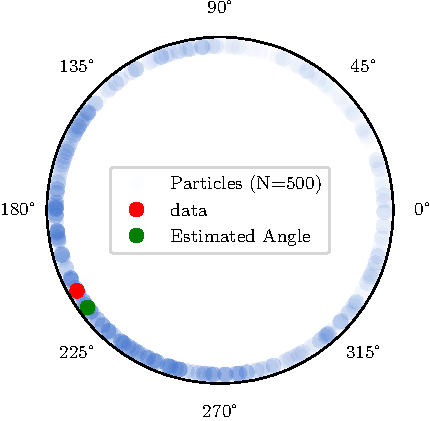
\includegraphics[width=0.47\textwidth]{actual_paper_graphs/particle_filter_example.pdf}\hfill
    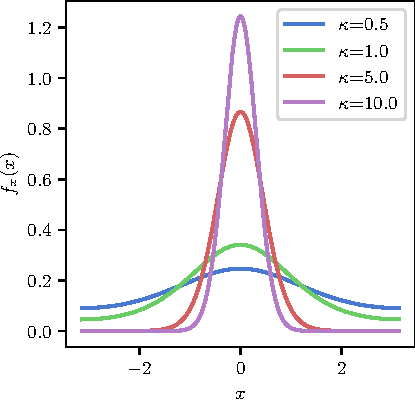
\includegraphics[width=0.47\textwidth]{actual_paper_graphs/von_mises_pdf.pdf}\hfill
    \caption{On the left, a particle filter example at a given timestep. The particles are colored according to weight, with the heaviest weights clustering around the data angle. On the right, the Von Mises distribution for various shape parameters ($\kappa$).}
    \label{fig:particle_filter_stuff}
\end{figure}

Particle filters suffer from what is called the "Degeneracy Problem", in which the weights become concentrated in a small number of the total particles. This is solved by resampling, a process in which low probability particles are replaced 
with higher probability particles. Detailing this problem and its solution is beyond our scope, but we used the \lstinline{systematic_resample} function from \lstinline{filterpy} to accomplish resampling.

As the particle filter keeps track of a large number of possible states which are distributed around the circle, it is much more flexible to nonlinear behavior. This is desirable in our case, as the source location may possibly reappear at any 
location in the state space. Unfortunately, the particle filter performs a similar number of computations for each individual particle as the Kalman filter performs in total. As we are using \lstinline{num_particles}, our particle filter takes \lstinline{n_particles} 
times as long to compute each step.

The Particle filter is defined with the following hyperparameters: 
\begin{itemize}
    \item \lstinline{K1} defines the analogous variance term for the distribution of the state noise.
    \item \lstinline{K2} defines the same for the measurements noise.
    \item \lstinline{N_particles} defines the number of particles the model employs.
    \item \lstinline{N_eff_particles} defines the minimum number of “effective” particles allowed before particles are resampled.
\end{itemize}

Similar to the Kalman filter, we tuned the hyperparameters \lstinline{K1},
\lstinline{K2},\newline \lstinline{N_particles}, and \lstinline{N_eff_particles} by performing a
gridsearch over many different possible values. A filter was constructed for each hyperparameter
combination, with its performance tested across several different datasets. We then chose the
hyperparameters that produced minimum average angular error over the different datasets. A similar
method was implemented for a robotics research paper as well see \cite{Oops}.

\section{Results and Analysis}
Here is a breakdown of the speed and accuracy of each filter (see Figure \ref{fig:all_filters}).

\subsection{Circular vs Naïve}
First, we compared the performance of the naive and circular Kalman filters in tracking a source moving continuously in a circle. The circular Kalman filter modification resulted in a marked improvement in behavior across the boundary between $360^{\circ}$ and $0^{\circ}$ as 
compared to the naive filter (see Figure \ref{fig:simple_kalman}). The Naive filter tended toward the arithmetic mean of $180^{\circ}$ for walking in a circle, while the circular Kalman filter accurately tracked the source around the entire circle.

\begin{figure}[htp]
    \centering
    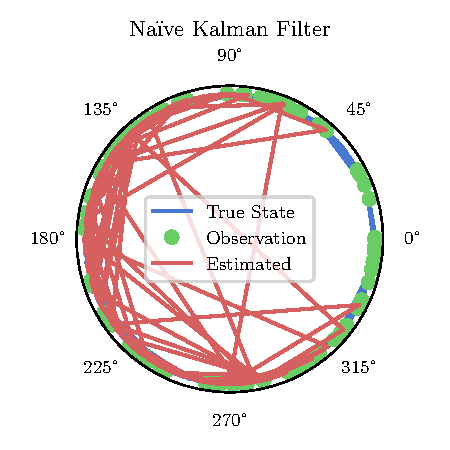
\includegraphics[width=0.47\textwidth]{non_altered_kalman.pdf}\hfill
    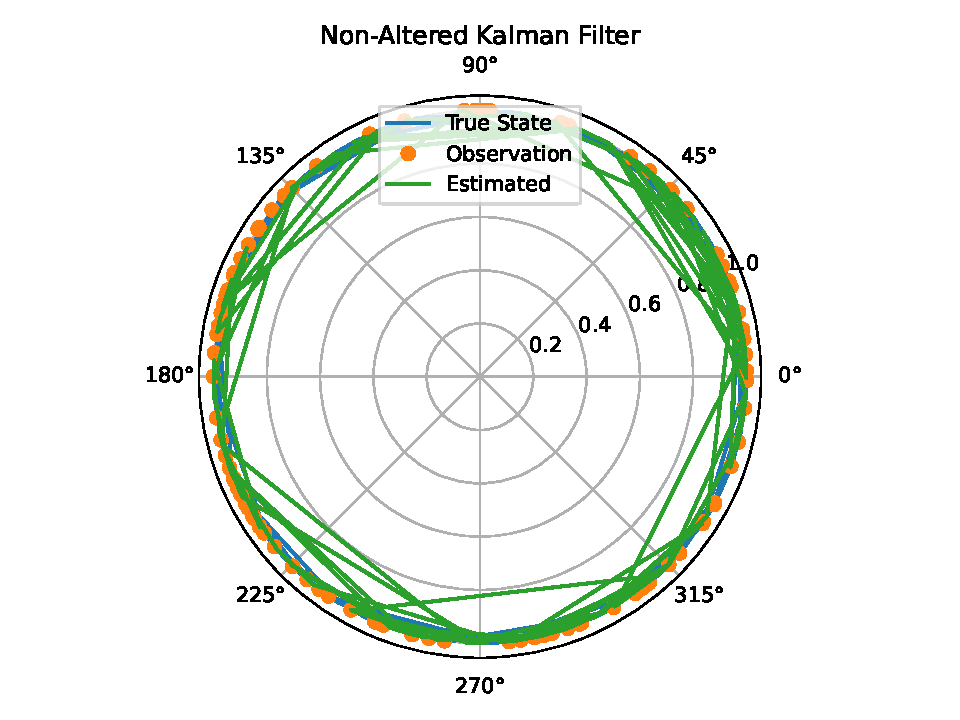
\includegraphics[width=0.47\textwidth]{altered_kalman.pdf}\hfill
    \caption{The naïve and circular Kalman Filter}
    \label{fig:simple_kalman}
\end{figure}

\subsection{Speed}
The Kalman filters ran in about $3$ to $5$ miliseconds on about 1 second worth of data. The Particle filter took about $125$ miliseconds on that dataset, so in total about $30$ times longer than the Kalman filters.
This means that all of our methods can be run in real time. 
\subsection{Accuracy}
We used average absolute angle error as our primary evaluation metric. This took the absolute value of the circular distance between the true state and predicted state at each time step and averaged it across time for the whole dataset. The performance of each filter varied depending on the dataset.
\subsubsection{White Noise at Constant Angle}
On the White Noise dataset, the Particle filter was the best filter, with about half the error of the Kalman filters. The error for the Kalman filters was almost exactly the same (.367 for Noncircular and .369 for Circular), which makes sense because the wraparound algorithm in the Circular Kalman filter was not used, making it behave exactly like the unmodified Kalman filter.
\subsubsection{Constant Angle with Engine Noise}
The Particle filter performed the best again on this data set, however the imporovement over the Kalman filters was not as large as it was with the White Noise data set. The error of the Particle filter was $\approx 25\%$ lower than the unmodified Kalman filter and was $\approx 40\%$ lower than the Circular Kalman filter. It is interesting to note that the unmodified Kalman filter performed significantly better than the Circular Kalman filter on this data set.
\subsubsection{Switching}
This is an artificial dataset created to simulate jumping between angles across $0^{\circ}$. The Naïve Kalman filter performed poorly on this dataset. The Circular Kalman and Particle filters performed much better, with the Particle filter being twice as accurate ($\mathrm{E}=0.199$ vs $\mathrm{E}=.392$) as the Circular Kalman filter.
\subsubsection{With Jump}
The Naïve Kalman filter performs better on this data set vs the Switching data set, but the results of the other two filters are the same.
\subsubsection{Wraparound}
The results of this dataset are the same as the previous dataset.
\subsubsection{The Best Filter}
The Circular Kalman and Particle filters both had consistent errors no matter the data set. The real trade off is whether we care more about speed or performance. The Particle filter was around twice as accurate, but it did take about 30 times longer to run. If computational efficiency is important, go with the Circular Kalman filter. If loacation accuracy is important, go with the Particle filter. The improvement in accuracy in the Particle filter is due to the lower variance compared with the Circular Kalman filter, as both responded to changes in angle measurements very quickly.

The researchers shared that due to limitations on reproducing angle-shifted sound accurately, that performance accurate to within approximately $15^{\circ}$ of accuracy is desirable. Of our algorithms, only the Particle filter consistently was within $15^{\circ}$ of accuracy.

\subsection{Hyperparameter tuning of Most Accurate Filter}

The particle filter has several model parameters as mentioned previously. We performed a grid search
to find the best filter for the engine dataset, see Figure \ref{fig:particle_hyperparam}.


\begin{figure}[htp]
    \centering
    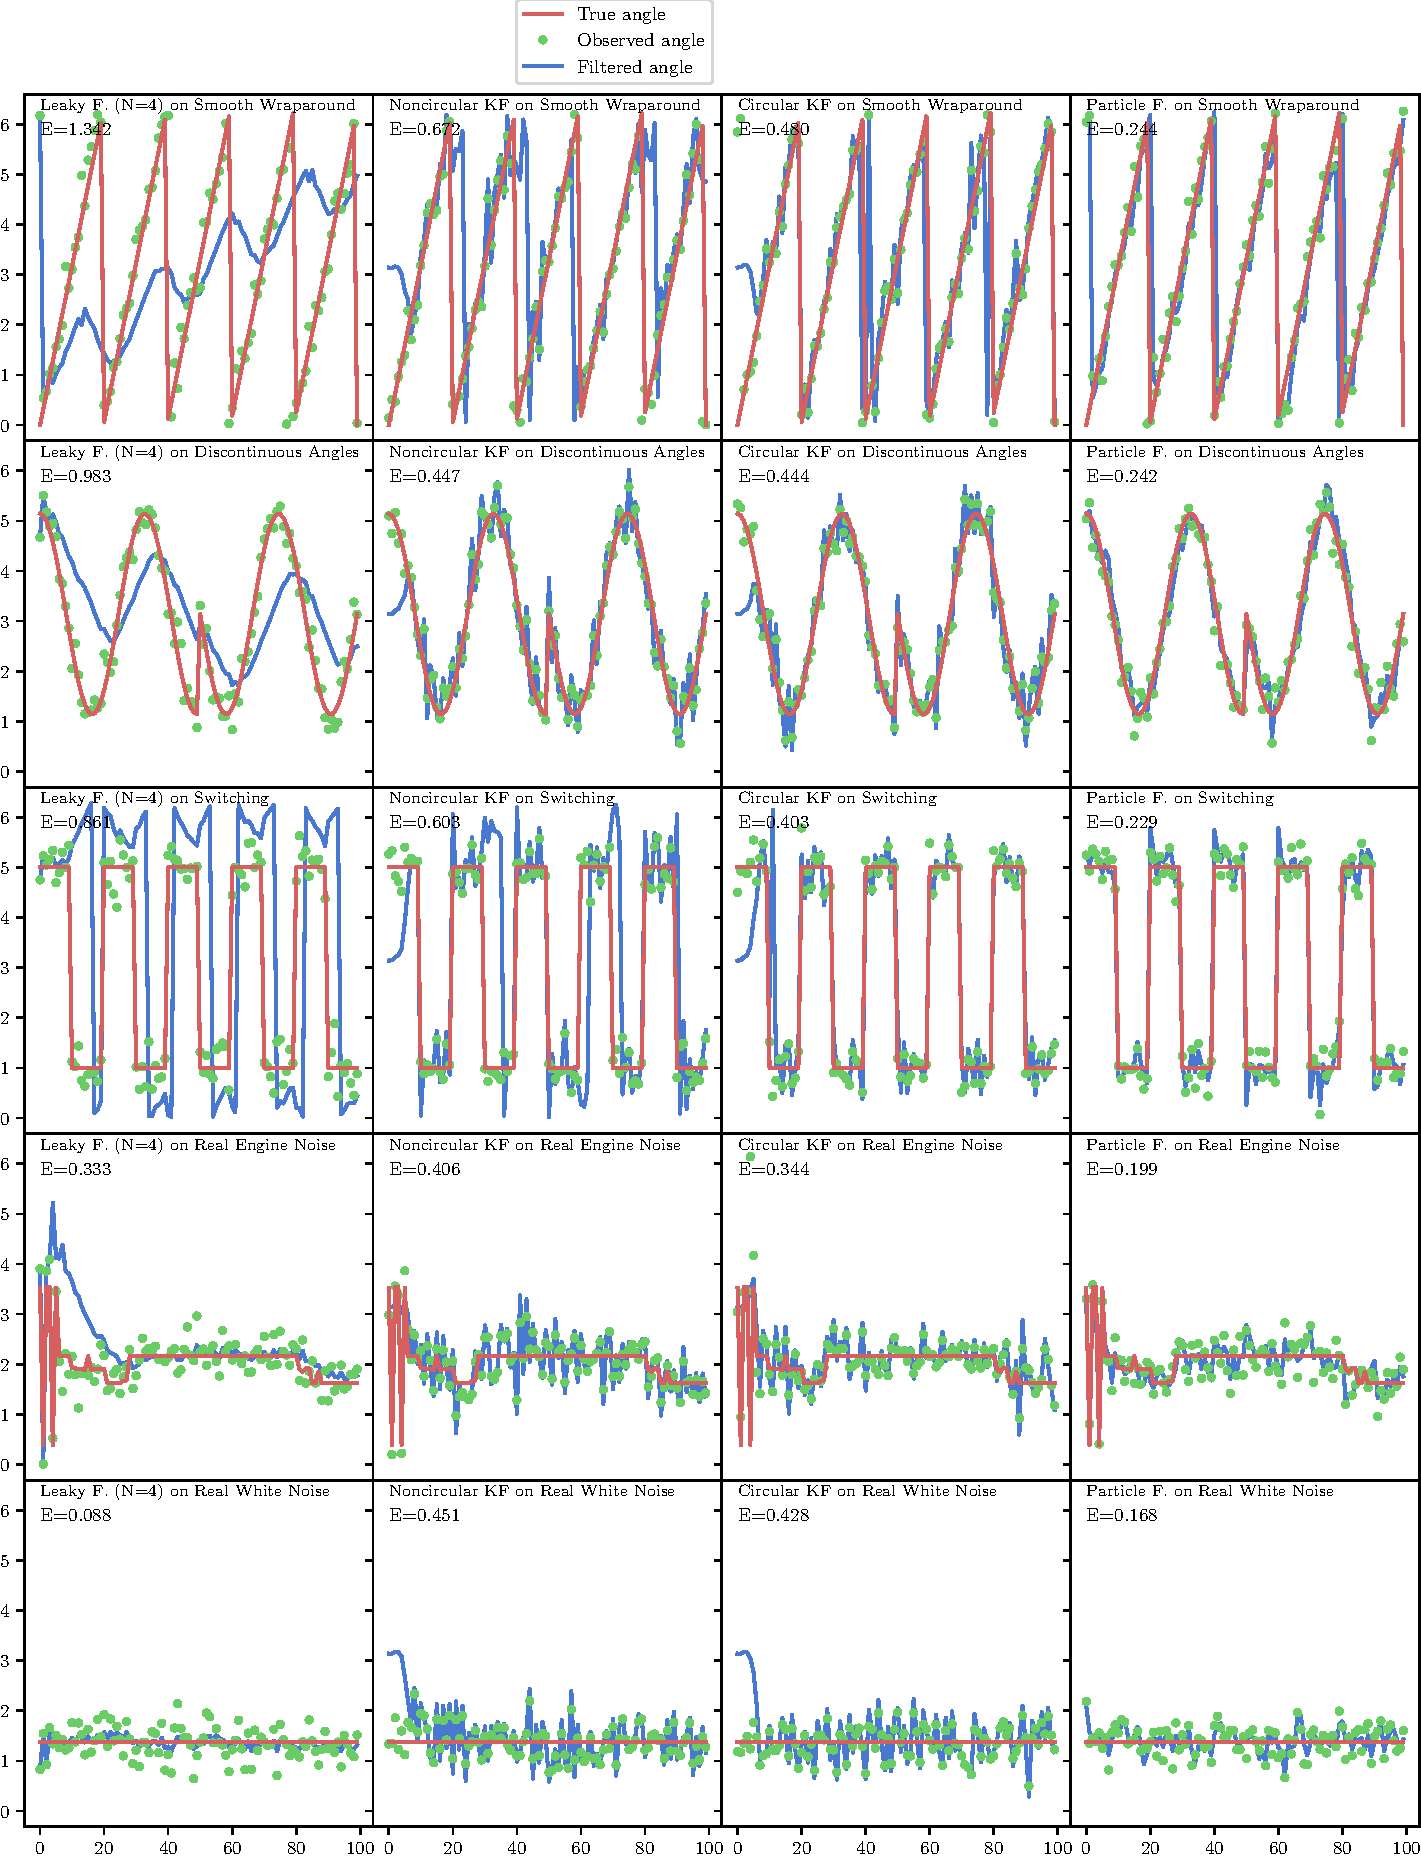
\includegraphics[width=.95\textwidth]{actual_paper_graphs/all.pdf}\hfill
    \caption{All filters, run on all datasets. Each row is a dataset, and each column is a type of filter. The green dots represent observations of the red true angle. The observations alone are filtered to produce the blue estimate angles.}
    \label{fig:all_filters}
\end{figure}



\begin{figure}[htp]
    \centering
    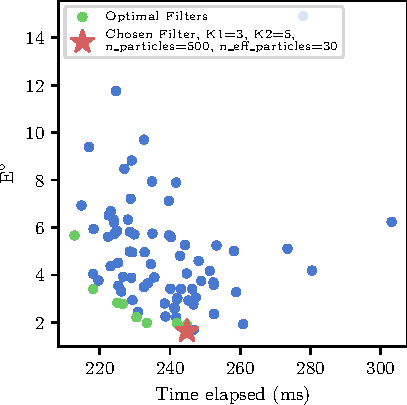
\includegraphics[width=1\textwidth]{actual_paper_graphs/gridsearch_particle_filter.pdf}\hfill
    \caption{Hyperparameter tuning of the Particle filter.}
    \label{fig:particle_hyperparam}
\end{figure}

\section{Ethical Considerations}
This project seeks to augment the safety of those outside the machinery by increasing the awareness of the machine operators. However, before deployment, this model must be 
shown to improve safety as much as or more than it increased the safety perception of the operators. Risk compensation “is a theory which suggests that people typically adjust 
their behavior in response to perceived levels of risk, becoming more careful where they sense greater risk and less careful if they feel more protected” \cite{Risk}. This should 
be accounted for before deploying these methods in the field to ensure that the model performs robustly enough to truly enhance overall safety, despite risk compensation. Furthermore, 
it should be emphasized that operators should still use sight and radio communication to identify nearby individuals, and that people near machinery must still exercise caution. 

\section{Conclusion}
Our goal was to improve robustness of the angle estimation by adapting filtering methods for use with circular data. We derived a very simple modification to the Kalman filter that 
allows it to work for circular data, and we implemented a particle filter using circular probability distributions. We found the particle filter and the circular Kalman filter suitable 
for angular data. The particle filter handles nonlinearities well but comes at a computational cost, while the circular Kalman filter is computationally efficient but suffers in 
accuracy in cases of strong nonlinearity. Due to the wraparound property of angular data, the unmodified Kalman filter is highly unsuitable for angular data. The particle 
filter and circular Kalman filter were both suitable, and can be adapted depending on the project’s needs.

For the BYU Acoustics project specifically, if the computational cost of the filtering step is a concern, we would recommend use of the circular Kalman filter for this project due to its low 
cost and accurate performance except in cases of strong nonlinearity. If more computational headroom is allowed, the particle filter would be ideal, as it performed well even in cases of 
nonlinearities. Furthermore, the utility of these methods extends to any field in which angle measurements are taken, including robotics, navigation, and astronomy. The hyperparameters of our 
methods can easily be modified to adjust accuracy, flexibility, and computational cost depending on what is needed for the given scenario. 




%%%%%%%%%%%%%%%%%%%%%%%%%%%%%%%%%%%%%
%% Bibliography below
%%%%%%%%%%%%%%%%%%%%%%%%%%%%%%%%%%%%%
\FloatBarrier % Keep the figures from being put after the bibliography
\newpage
%% If using bibtex, leave this uncommented
%\bibliography{refs} %if using bibtex, call your bibtex file refs.bib
\bibliographystyle{alpha}

%% If not using bibtex, comment out the previous two lines and uncomment those below
\begin{thebibliography}{99}
\bibitem{Research} G. Kurz, I. Gilitschenski and U. D. Hanebeck, "Recursive nonlinear filtering for angular data based on circular distributions," \textit{2013 American Control Conference}, Washington, DC, USA, 2013, pp. 5439-5445, doi: 10.1109/ACC.2013.6580688.
\bibitem{V3} The ACME Volume 3 Textbook
\bibitem{V3 Lab Manual} J. Humpherys and T. Jarvis, "Labs for Foundations of Applied Mathematics, Volume 3, Modeling with Uncertainty and Data."
\bibitem{Particle} Labbe, Roger. “Kalman and Bayesian Filters in Python”.
\bibitem{Risk} Masson, Maxime; Lamoureux, Julie; de Guise, Elaine (October 2019). "Self-reported risk-taking and sensation-seeking behavior predict helmet wear amongst Canadian ski and snowboard instructors". \textit{Canadian Journal of Behavioural Science.} 52 (2): 121–130. doi:10.1037/cbs0000153. S2CID 210359660.
\bibitem{Oops} I. Marković and I. Petrović, "Speaker localization and tracking with a microphone array on a mobile robot using von Mises distribution and particle filtering," \textit{Robotics and Autonomous Systems}, Volume 58, Issue 11, 2010, pp. 1185-1196, doi: 10.1016/j.robot.2010.08.001
\end{thebibliography}

\end{document}